\documentclass[12pt,a4paper]{report}
\usepackage[utf8]{inputenc}
\usepackage[german]{babel}
\usepackage[T1]{fontenc}
\usepackage{amsmath}
\usepackage{amsfonts}
\usepackage{amssymb}
\usepackage{lmodern}
\usepackage{authoraftertitle}
\usepackage{fancyhdr}
\usepackage[final]{graphicx}
\DeclareGraphicsExtensions{.pdf,.png,.jpg}
\usepackage{color}

% header
\pagestyle{fancy}
\fancyhead[L]{\today}
\fancyhead[R]{DezSys - Verteilte Datenbanken}

%footer
\fancyfoot[L]{Ayvazyan, Haidn}
\fancyfoot[C]{5A HIT}
\fancyfoot[R]{Seite \thepage/\pageref{LastPage}}

\date{10.10.2014}
\author{Ari Ayvazyan, Martin Haidn}
\title{Verteilte Datenbanken}

\begin{document}
\maketitle
\tableofcontents
	\chapter{Angabe}
		\section{Einführung}	
			Es soll eine Verteilte Datenbank mit Oracle XE realisiert werden. Die Hauptaufgabe ist es herauszufinden wie man eine verteilte Datenbank erstellt. Die einzige Informationsquelle ist das weite Netz, allem voran die Oracle Dokumentation Site. Der komplette Datenbankentwurf für ein
			verteiltes Oracle-DBS soll erstellt werden. Zu verwenden ist dabei eine geeignete
			Fragmentierungsmethode! Die einzelnen Schritte sind zu dokumentieren, und Abfragen
			durchzuführen, die eine Connection auf die verteilte Instanz nötig machen!
		\section{Anforderungsanalyse}
			Die MensaAustria plant die Erstellung einer Datenbank zur Vereinfachung der Arbeitsabläufe. Dabei
			ist zu beachten, dass jede Universität ihre eigene Verwaltung bekommt, jedoch von einer Stelle
			geleitet wird.\\\\
			Eine Speise hat eine eindeutige Nummer, einen Namen und einen Typ (Vorspeise, Hauptspeise,
			Nachspeise). Eine Speise besteht aus mehreren Zutaten, wobei die Menge der einzelnen Zutaten
			gespeichert werden muss.\\\\
			Eine Zutat hat eine eindeutige Nummer, einen Namen, eine Einheit (kg, Liter, etc.), einen Preis pro
			Einheit und einen bzw. mehrere Lieferanten, von denen die Adresse und eine eindeutige
			UIDNummer bekannt sind. Weiters wird die Kundennummer der Mensa beim jeweiligen Lieferanten
			vermerkt. Der Lagerbestand wird ebenfalls modelliert. Dazu sind von jeder Zutat die Anzahl der
			Einheiten, die momentan vorrätig sind, bekannt. Wenn eine Zutat nicht mehr vorrätig ist, so wird der
			Bestand auf 0 gesetzt.\\\\
			Im Falle einer Bestellung werden ein bzw. mehrere Zutaten bei einem bestimmten Lieferanten
			bestellt. Die Bestellung hat eine eindeutige Bestellnummer, ein Bestelldatum, ein voraussichtliches
			Lieferdatum. Die einzelnen Zutaten sind die Bestellposten, die eine pro Bestellung eindeutige
			Nummer haben, und bei denen die bestellte Menge und der verhandelte Preis gespeichert werden.
			Zu jeder Bestellung gibt es nach erfolgter Lieferung eine Rechnung, die verbucht werden muss.
			Rechnungen beziehen sich auf genau eine Bestellung. Dabei wird die eindeutige Rechnungsnummer,
			die Bankverbindung und die Rechnungssumme gespeichert, wobei letztere vom Bestellpreis
			differieren kann, wenn ein Skonto anfällt.\\\\
			Ein Menü hat einen eindeutigen Namen, einen Preis und es ist gespeichert, aus welchen
			(verschiedenen) Speisen ein Menü besteht. Eine Speise kann selbstverständlich in mehreren Menüs
			vorkommen.\\\\
			Um eine zu große Eintönigkeit in der Menüabfolge zu vermeiden, wird weiters gespeichert, an
			welchen Tagen welche Menüs serviert wurden. An jedem Tag werden genau drei Menüs serviert.
	\chapter{Datenbank Entwurf}
		\section{Diagramm}
			\begin{figure}[h!]
				\centering
				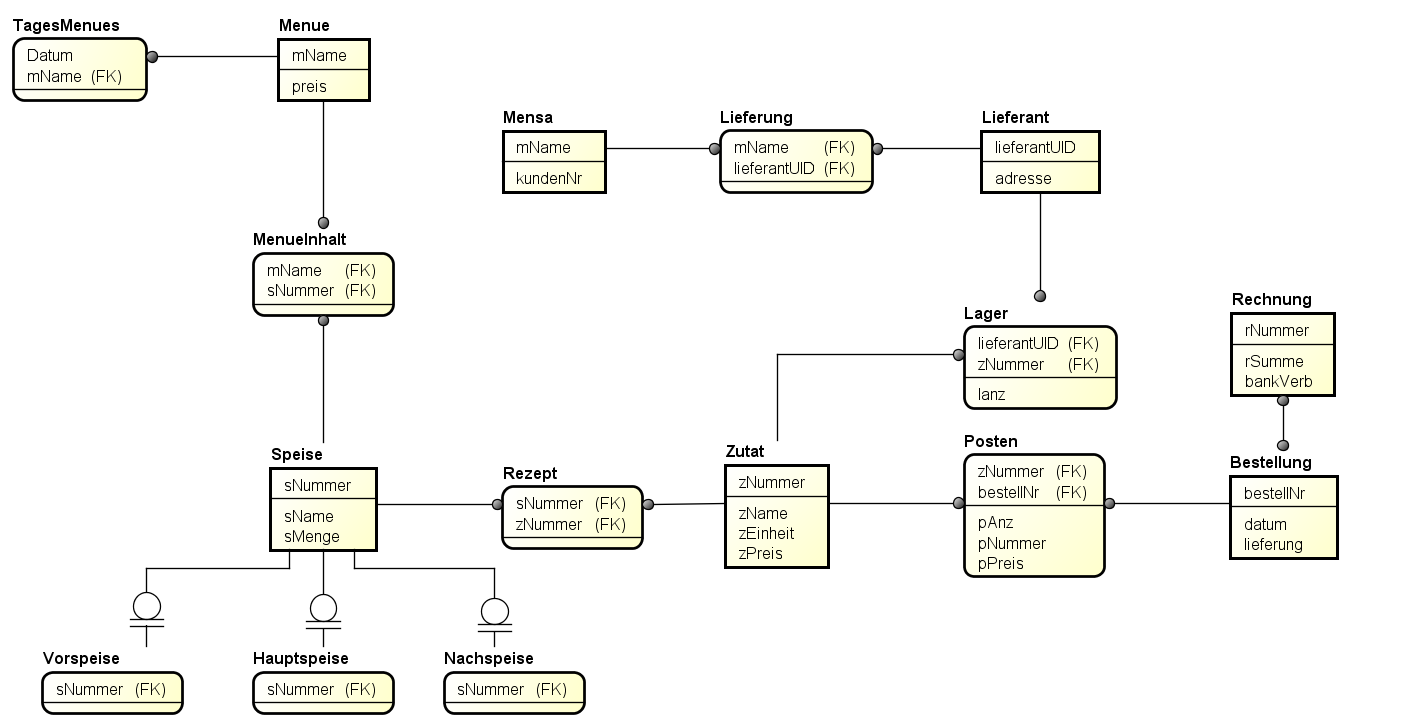
\includegraphics[width=1\linewidth]{ERD/MensaEr.png}
				\caption{ERD}
				\label{fig:MensaEr.png}
			\end{figure}
		\section{Konfiguration}
	\chapter{Fragmentierung}
		\section{Horizontal}
			Die Mensa scheint perfekt für eine horizontale Fragmentierung geeignet, hier würden die Daten je nach geografischer Lage des typischen Zugriffsorts horizontal getrennt.
		\section{Vertikal}
			Vertikale Trennung scheint in diesem Beispiel weniger sinnvoll.
	\chapter{Abfragen}
		Database links are the invisible glue that makes location transparency possible.
	\chapter{Quellen}
		http://oreilly.com/catalog/ordistsys/chapter/ch01.html
\end{document}
